\documentclass{article}

\PassOptionsToPackage{numbers,sort&compress}{natbib}
\usepackage[preprint]{neurips}
\usepackage[utf8]{inputenc}
\usepackage[T1]{fontenc}
\usepackage{hyperref}
\usepackage{url}
\usepackage{booktabs}
\usepackage{amsfonts}
\usepackage{nicefrac}
\usepackage{microtype}
\usepackage{xcolor}
\usepackage{graphicx}
\usepackage{subcaption}
\usepackage{multirow}
\usepackage{array}
\usepackage{float}
\usepackage{adjustbox}
\usepackage{amsthm}
\usepackage{amsmath}
\usepackage{amssymb}
\usepackage{mathtools}
\usepackage{enumitem}
\usepackage{algorithm}
\usepackage{algpseudocode}
\usepackage{bbm}

\title{PRISM: Post-hoc Domain Generalization via Worst-Case Regret over Hidden Source-Supported Subpopulations}
\author{Anonymous Authors}

\newtheorem{theorem}{Theorem}
\newtheorem{proposition}{Proposition}
\newtheorem{lemma}{Lemma}
\newtheorem{corollary}{Corollary}
\newtheorem{definition}{Definition}
\newtheorem{assumption}{Assumption}
\newtheorem{remark}{Remark}

\newcommand{\RR}{\mathbb{R}}
\newcommand{\EE}{\mathbb{E}}
\newcommand{\PP}{\mathbb{P}}
\newcommand{\cA}{\mathcal{A}}
\newcommand{\cC}{\mathcal{C}}
\newcommand{\cD}{\mathcal{D}}
\newcommand{\cI}{\mathcal{I}}
\newcommand{\cQ}{\mathcal{Q}}
\newcommand{\cR}{\mathcal{R}}
\newcommand{\cS}{\mathcal{S}}
\newcommand{\cT}{\mathcal{T}}
\newcommand{\cU}{\mathcal{U}}
\newcommand{\cV}{\mathcal{V}}
\newcommand{\argmin}{\operatorname*{arg\,min}}
\newcommand{\argmax}{\operatorname*{arg\,max}}
\newcommand{\CVaR}{\operatorname{CVaR}}
\newcommand{\Top}{\operatorname{Top}}
\newcommand{\KL}{\operatorname{KL}}
\newcommand{\simplex}{\Delta}
\newcommand{\TBD}{\textbf{TBD}}
\newcommand{\prism}{\textup{\textsc{PRISM}}}
\newcommand{\swad}{\textup{\textsc{SWAD}}}
\newcommand{\diwa}{\textup{\textsc{DiWA}}}
\newcommand{\miro}{\textup{\textsc{MIRO}}}
\newcommand{\erm}{\textup{\textsc{ERM}}}
\newcommand{\iid}{i.i.d.}
\newcommand{\ood}{OOD}
\newcommand{\norm}[1]{\left\lVert #1 \right\rVert}
\newcommand{\braces}[1]{\left\{ #1 \right\}}
\newcommand{\paren}[1]{\left( #1 \right)}
\newcommand{\bracks}[1]{\left[ #1 \right]}
\newcommand{\loss}{\ell}
\newcommand{\1}{\mathbbm{1}}

\begin{document}

\maketitle

\begin{abstract}
Single-run post-hoc selection has become one of the most practical routes to domain generalization because it can be attached to a strong empirical-risk-minimization pipeline without retraining. Several influential post-hoc approaches, however, still optimize proxies: flat intervals along a trajectory, checkpoint-wise stability scores, or raw worst-case loss surrogates. This paper studies a stricter alignment between theory and deployment. We propose \textbf{\prism{}} (\textbf{P}ost-hoc \textbf{R}egret on \textbf{I}mplicit \textbf{S}ubpopulations of \textbf{M}odel soups), a domain-label-free post-hoc selector whose decision variable is the averaged-state soup scored by the second stage: a uniform average of an anchor-screened subset of checkpoints from one dense run. \prism{} selects that soup by minimizing worst-case regret to the best feasible soup across all sufficiently large hidden source-supported subpopulations. The objective has an explicit top-$\alpha$-mean and empirical-\(\CVaR\) characterization, is exact for the fully enumerated scored action family, and yields a direct target-regret certificate under source-supported hidden-subpopulation shift. We prove interval-family domination, consistency of the second-stage selector conditional on a fixed candidate family, monotonic robustness certificates, exact optimality of the exhaustive solver over the scored action family, and constructive complementarity results showing when noncontiguous soups are strictly necessary. The experimental section records the evaluation protocol together with exact published benchmark frontiers from prior work.
\end{abstract}

\section{Introduction}

Domain generalization (DG) asks for a model that performs well on an unseen target environment using only source data at training time. In practice, the most durable DG ideas are often the ones that leave the training recipe largely intact and modify only how the final model is selected. This has made post-hoc single-run selectors especially appealing: one can train a standard source-pooled model, save dense checkpoints, and then choose one deployable predictor after training has already finished.

That practical appeal has already translated into strong published results. On the standard DomainBed ResNet-50 benchmark suite, an interval-based flat-minima selector improves the average \ood{} accuracy of \erm{} from \(63.3\) to \(66.9\) across PACS, VLCS, OfficeHome, TerraIncognita, and DomainNet \citep{cha2021swad}. A pretraining-aware regularizer combined with the same post-hoc interval selector reaches \(68.1\) on the same benchmark family \citep{cha2022miro}. Weight averaging, model soups, and diversity-aware analyses all reinforce the same empirical message: the final predictor is often not the last checkpoint \citep{izmailov2018swa,wortsman2022soups,rame2022diwa}.

Still, a theoretical gap remains. Interval-based selectors are motivated by flatness and robust empirical risk, but they do not directly optimize the final theoretical object they are said to target. Model soups and trajectory averages often rely on locality assumptions or validation heuristics, but the selected predictor is still one concrete soup. If theory is going to govern the method rather than merely rationalize it after the fact, the post-hoc objective should be written directly over the soup family that is actually scored during selection.

A direct formulation follows. \textbf{\prism{}} denotes \textbf{P}ost-hoc \textbf{R}egret on \textbf{I}mplicit \textbf{S}ubpopulations of \textbf{M}odel soups. The central idea is:
\begin{quote}
\textbf{A robust post-hoc soup is one whose performance has small worst-case regret to the best feasible soup on every sufficiently large hidden source-supported subpopulation.}
\end{quote}

The resulting selector is domain-label-free: it uses only a pooled source holdout split, not source-domain identities. It is also exact with respect to the second-stage averaged-state family it scores. A dense trajectory is reduced to an anchor-screened low-loss candidate pool. The action space is the family of uniform soups over feasible subsets of that pool. A capped adversary ranges over sufficiently large hidden subpopulations of the pooled source support. For each candidate soup, \prism{} measures regret relative to the best feasible soup for that adversarially reweighted support and selects the soup with the smallest worst-case regret.

This choice of primitive has two advantages. First, regret is more stable than raw risk under heterogeneous subgroup difficulty, a point formalized in minimax-regret learning under distribution shift \citep{agarwal2022mro}. Second, sufficiently large hidden subpopulation shifts provide a direct domain-label-free uncertainty family, closely related to worst-case subpopulation evaluation and robust learning without observed group identities \citep{li2021worstcase,hashimoto2018fairness,lahoti2020fairness}. The resulting objective is aligned with the scored action family: the selector computes losses of actual uniform soups, evaluates capped-adversary regret over the support set, and returns the global empirical minimizer over that scored family whenever it is fully enumerated.

The paper makes four contributions.
\begin{enumerate}[leftmargin=1.4em]
    \item We formulate \prism{}, a single-run post-hoc DG method whose decision variable is the averaged-state soup scored by the second stage and whose uncertainty family is defined by hidden source-supported subpopulations rather than observed domain labels.
    \item We derive an exact finite-sample characterization of the empirical objective as a maximum of top-$\alpha$ means, equivalently an empirical-\(\CVaR\) regret over pairwise action gaps.
    \item We prove a target-regret certificate under hidden-subpopulation shift, interval-family domination for any interval-restricted post-hoc selector embedded in the same feasible action family, consistency of the second-stage selector conditional on a fixed candidate family, monotonic robustness certificates, and constructive complementarity theorems showing when noncontiguous soups are strictly required.
    \item We record an experimental protocol and exact published benchmark context from prior work, together with structured reporting tables for the empirical evaluation.
\end{enumerate}

\begin{figure}[t]
    \centering
    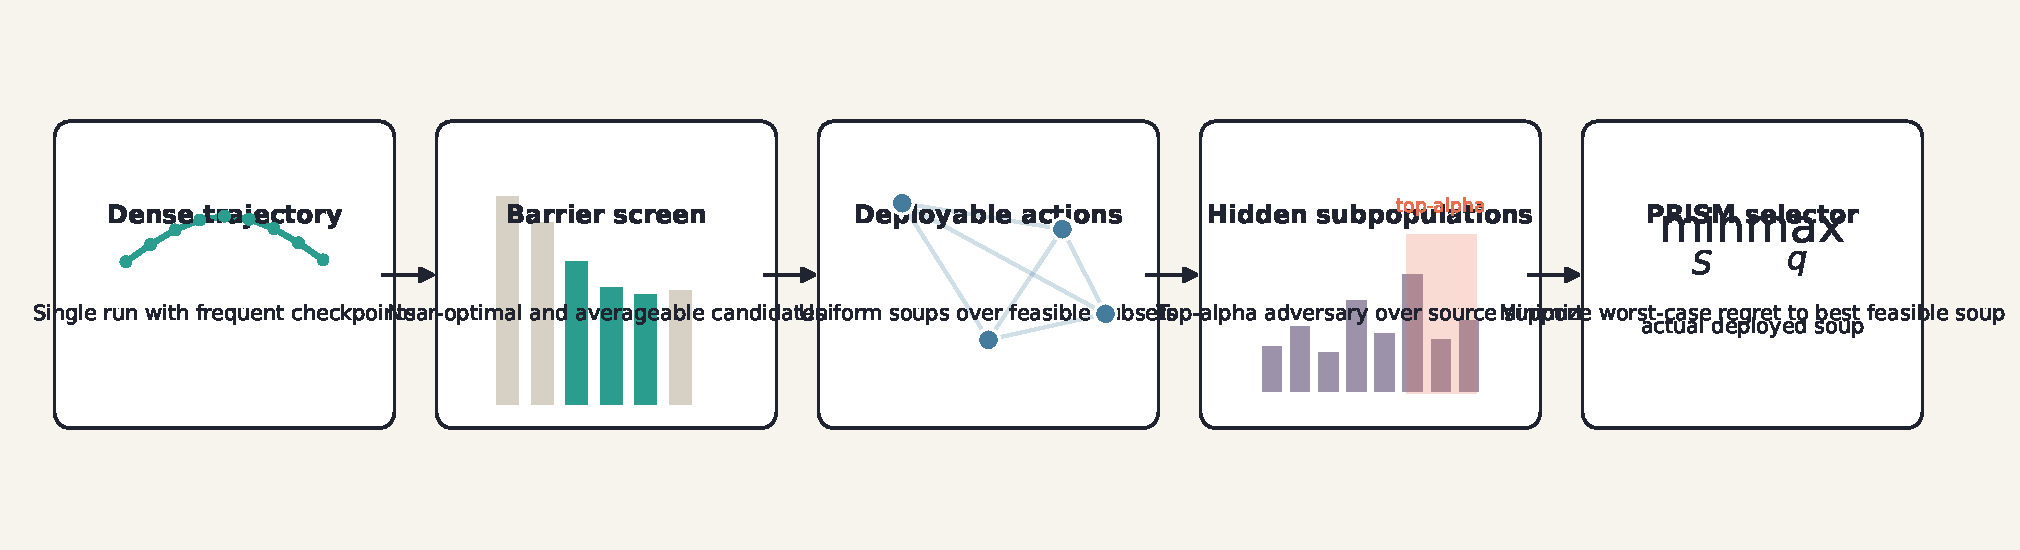
\includegraphics[width=\linewidth]{figures/prism_overview.pdf}
    \caption{\textbf{\prism{} overview.} A dense single-run trajectory is reduced to a low-loss, anchor-screened candidate pool. The action space consists of uniform soups over feasible subsets of that pool. \prism{} then chooses the soup with smallest worst-case regret to the best feasible soup over hidden source-supported subpopulations of the pooled support split.}
    \label{fig:overview}
\end{figure}

\section{Related Work}

\paragraph{Post-hoc DG and interval-based selectors.}
Flat-minima-inspired post-hoc selectors showed that one can obtain large DG gains without changing the base training algorithm \citep{cha2021swad}. Their core insight is important: late-trajectory averages can be far more robust than a single checkpoint. Yet the selected action family is still constrained to contiguous intervals and validation heuristics. \prism{} keeps the single-run post-hoc setting but replaces the interval heuristic with an exact objective over a larger scored action family.

\paragraph{Weight averaging, connectivity, and soups.}
Stochastic weight averaging, mode connectivity, and model soups established that averaging weights can be effective when models remain in a connected low-loss region \citep{izmailov2018swa,garipov2018fge,frankle2020linear,wortsman2022soups}. \diwa{} clarified the \ood{} picture by decomposing the expected error of weight averaging into bias, variance, covariance, and locality terms \citep{rame2022diwa}. \prism{} preserves a locality screen through an anchor-based barrier heuristic, but it moves the optimization target from a weight-space proxy to regret over actual soups.

\paragraph{Distributionally robust and subgroup-robust learning.}
Distributionally robust optimization studies predictors that minimize worst-case risk over ambiguity sets around a nominal distribution \citep{duchi2016fdiv,duchi2021learning}. Group-robust and fairness-oriented methods use related adversarial reweightings to protect minority groups or latent subpopulations \citep{hashimoto2018fairness,lahoti2020fairness,sagawa2020groupdro}. The closest adjacent perspective to ours is worst-case subpopulation evaluation \citep{li2021worstcase}, which studies performance over all sufficiently large subpopulations defined by core attributes. \prism{} adapts that hidden-subpopulation viewpoint to post-hoc model selection.

\paragraph{Regret under distribution shift.}
Minimax regret optimization argues that regret, rather than raw worst-case risk, is the more stable object under heterogeneous noise or varying subgroup difficulty \citep{agarwal2022mro}. That distinction is central here. In a post-hoc action family, worst-case risk alone can prefer soups that are uniformly conservative but not actually close to the best feasible soup on hard subpopulations. \prism{} optimizes worst-case regret instead.

\paragraph{Pretraining-aware DG.}
Pretraining-aware DG methods such as \miro{} are complementary to post-hoc selectors: they improve the underlying trajectory, while post-hoc selection chooses one final predictor from that trajectory \citep{cha2022miro}. The present paper focuses exclusively on the latter problem.

\section{Problem Setup}
\label{sec:setup}

We consider multiclass classification in the standard single-run DG setting. A base learning algorithm produces dense checkpoints
\[
    \{\theta_t\}_{t=1}^{K}.
\]
Post-hoc selection uses two labeled pooled source holdout sets:
\begin{itemize}[leftmargin=1.4em]
    \item a \emph{validation} split \(\cV = \{(x_j,y_j)\}_{j=1}^{n_V}\), used only for low-loss filtering and barrier tests, and
    \item a \emph{support} split \(\cU = \{(x_i,y_i)\}_{i=1}^{n}\), used only for robust post-hoc selection.
\end{itemize}
Neither split uses source-domain labels. In the implementation, both are constructed by pooling the source holdout examples and then partitioning that pool into validation and support subsets.

For checkpoint \(\theta_t\), let \(p_t(x)\in\simplex^{C-1}\) denote the predicted class-probability vector. Fix a probability floor \(\varepsilon_p\in(0,1)\). The pooled validation loss is
\begin{equation}
    L_{\cV}(\theta_t)
    \triangleq
    \frac{1}{n_V}\sum_{j=1}^{n_V} -\log \max\braces{p_t(x_j)_{y_j}, \varepsilon_p}.
    \label{eq:val_loss}
\end{equation}

We choose the anchor checkpoint by pooled validation loss:
\begin{equation}
    a \in \argmin_{1\le t\le K} L_{\cV}(\theta_t).
    \label{eq:anchor}
\end{equation}

Locality is screened using a pooled anchor-based interpolation barrier. For a fixed interpolation grid \(\cA \subset [0,1]\),
\begin{equation}
    B(t,a)
    \triangleq
    \max_{\lambda\in \cA}
    L_{\cV}\big((1-\lambda)\theta_a + \lambda \theta_t\big)
    -
    \max\braces{L_{\cV}(\theta_a), L_{\cV}(\theta_t)}.
    \label{eq:barrier}
\end{equation}
The candidate pool is
\begin{equation}
    \cC
    \triangleq
    \braces{
        t :
        L_{\cV}(\theta_t)\le L_{\cV}^\star + \varepsilon,\;
        B(t,a)\le \tau
    },
    \qquad
    L_{\cV}^\star = \min_t L_{\cV}(\theta_t).
    \label{eq:candidate_pool}
\end{equation}

The post-hoc action family is the set of uniform soups over feasible subsets of the anchor-screened candidate pool.
\begin{definition}[Feasible soup action family]
Fix a cardinality budget \(M\ge 1\). The feasible action set is
\begin{equation}
    \cS_M
    \triangleq
    \braces{
        S \subseteq \cC : 1 \le |S| \le M
    }.
    \label{eq:action_set}
\end{equation}
The scored soup associated with action \(S\in\cS_M\) is
\begin{equation}
    \bar{\theta}_S
    \triangleq
    \frac{1}{|S|} \sum_{t\in S} \theta_t.
    \label{eq:uniform_soup}
\end{equation}
\end{definition}

This definition matches the second-stage selector: \prism{} never optimizes a predictive mixture or a relaxed continuous soup that is not actually scored. In implementations with batch-normalization layers, an optional post-selection BN re-estimation pass may be applied to the winning soup before final evaluation; the exact objective analyzed here is the pre-refresh scored family in Eq.~\eqref{eq:uniform_soup}.

For each support example \(z_i=(x_i,y_i)\in \cU\), define the clipped action loss
\begin{equation}
    \loss_i(S)
    \triangleq
    -\log \max\braces{p_{\bar{\theta}_S}(x_i)_{y_i}, \varepsilon_p}.
    \label{eq:empirical_action_loss}
\end{equation}
This yields the deterministic bound
\begin{equation}
    0 \le \loss_i(S) \le L_{\max},
    \qquad
    L_{\max} \triangleq -\log \varepsilon_p.
    \label{eq:lmax}
\end{equation}
The support loss vector of \(S\) is
\(
    \loss(S) = \paren{\loss_1(S),\ldots,\loss_n(S)} \in \RR^n.
\)

\section{\prism{}: Hidden-Subpopulation Regret over Scored Soup Actions}
\label{sec:method}

\subsection{Capped adversaries and empirical regret}

Let \(\alpha\in(0,1]\) denote the minimum subpopulation mass that we wish to protect. Define the capped adversarial simplex
\begin{equation}
    \cQ_\alpha^n
    \triangleq
    \braces{
        q \in \simplex^n :
        q_i \le \frac{1}{\alpha n}
        \;\;\forall i
    }.
    \label{eq:capped_simplex}
\end{equation}
This is the finite-sample version of the hidden-subpopulation family: the adversary may concentrate mass on any sufficiently large subset of support examples, but cannot collapse onto a vanishing number of points.

For any action \(S\in\cS_M\), define its empirical hidden-subpopulation regret by
\begin{equation}
    \widehat{\Psi}_\alpha(S)
    \triangleq
    \sup_{q \in \cQ_\alpha^n}
    \left[
        \sum_{i=1}^{n} q_i \loss_i(S)
        -
        \min_{S' \in \cS_M}
        \sum_{i=1}^{n} q_i \loss_i(S')
    \right].
    \label{eq:empirical_prism}
\end{equation}
The \prism{} selector is the exact empirical minimizer
\begin{equation}
    \widehat{S}_\alpha
    \in
    \argmin_{S\in\cS_M} \widehat{\Psi}_\alpha(S).
    \label{eq:prism_selector}
\end{equation}

The objective in Eq.~\eqref{eq:empirical_prism} is the exact second-stage quantity used by the selector. It enumerates the feasible soups, evaluates the support loss vector of each scored soup, and chooses the soup whose worst-case regret is smallest.

\subsection{\texorpdfstring{Exact top-\(\alpha\) and empirical-\(\CVaR\) characterization}{Exact top-alpha and empirical-CVaR characterization}}

For \(v\in\RR^n\), let \(v_{(1)}\ge \cdots \ge v_{(n)}\) denote its sorted entries. Define the finite-sample top-\(\alpha\) mean by
\begin{equation}
    \Top_\alpha(v)
    \triangleq
    \sup_{q\in\cQ_\alpha^n} \sum_{i=1}^{n} q_i v_i.
    \label{eq:top_alpha_def}
\end{equation}

\begin{proposition}[Exact top-\(\alpha\) form of the empirical objective]
\label{prop:top_alpha}
For any \(S\in\cS_M\),
\begin{equation}
    \widehat{\Psi}_\alpha(S)
    =
    \max_{S' \in \cS_M}
    \Top_\alpha\!\big(\loss(S)-\loss(S')\big).
    \label{eq:prism_top_alpha}
\end{equation}
Moreover, if \(m=\alpha n\), \(k=\lfloor m\rfloor\), and \(\rho = m-k\), then
\begin{equation}
    \Top_\alpha(v)
    =
    \begin{cases}
        v_{(1)}, & m \le 1, \\[0.3em]
        \dfrac{1}{m}\left(\sum_{j=1}^{k} v_{(j)} + \rho\,v_{(k+1)}\right), & 1 < m < n, \\[0.7em]
        \dfrac{1}{n}\sum_{j=1}^{n} v_j, & m \ge n.
    \end{cases}
    \label{eq:top_alpha_closed}
\end{equation}
Equivalently,
\begin{equation}
    \Top_\alpha(v)
    =
    \inf_{\eta\in\RR}
    \bracks{
        \eta + \frac{1}{\alpha n}\sum_{i=1}^{n}(v_i-\eta)_+
    },
    \label{eq:top_alpha_cvar}
\end{equation}
so the empirical hidden-subpopulation regret is an exact empirical-\(\CVaR\) regret over pairwise action gaps.
\end{proposition}

The importance of Proposition~\ref{prop:top_alpha} is methodological. The selector is not optimizing a proxy that only resembles the deployed soup. The exact support-level objective of the second-stage problem is a maximum of top-\(\alpha\) pairwise regret means, equivalently a maximum of empirical-\(\CVaR\) regret gaps.

\begin{figure}[t]
    \centering
    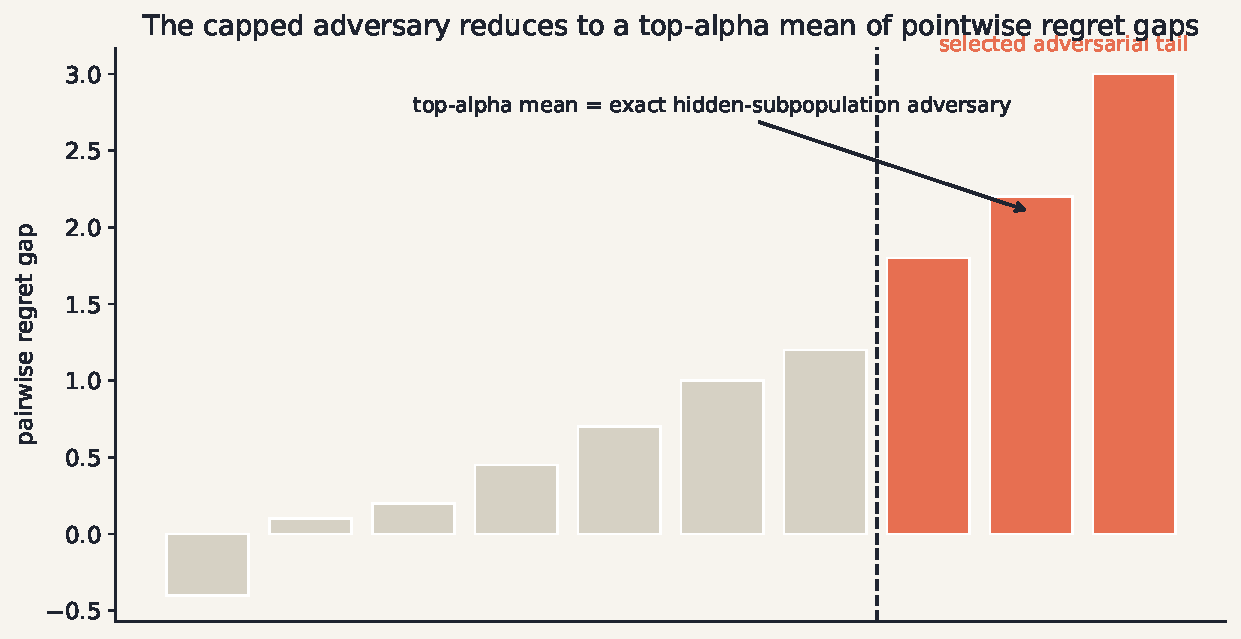
\includegraphics[width=0.87\linewidth]{figures/top_alpha_regret_geometry.pdf}
    \caption{\textbf{Exact adversary geometry.} For a fixed candidate soup \(S\) and witness soup \(S'\), the capped adversary selects the highest pairwise regret tail. This is the exact empirical objective used by \prism{}, not a surrogate.}
    \label{fig:top_alpha}
\end{figure}

\subsection{Exact exhaustive selector}

The second-stage selector uses exact exhaustive search over \(\cS_M\) whenever the scored family is small enough to be fully enumerated. Because the candidate pool is anchor-screened and \(M\) is small, this is tractable for the moderate action families considered here.

\begin{algorithm}[t]
\caption{\prism{} exact post-hoc selector}
\label{alg:prism}
\begin{algorithmic}[1]
\Require Dense checkpoints \(\{\theta_t\}_{t=1}^{K}\), pooled validation split \(\cV\), pooled support split \(\cU\), thresholds \(\varepsilon,\tau\), barrier grid \(\cA\), subpopulation mass \(\alpha\), soup budget \(M\)
\State Choose anchor \(a\) by Eq.~\eqref{eq:anchor}
\State Build candidate pool \(\cC\) by Eq.~\eqref{eq:candidate_pool}
\State Enumerate all feasible subset actions \(\cS_M\) from Eq.~\eqref{eq:action_set}
\For{each \(S\in\cS_M\)}
    \State Materialize the scored soup \(\bar{\theta}_S\) from Eq.~\eqref{eq:uniform_soup}
    \State Evaluate \(\loss(S)\) on the pooled support split \(\cU\)
\EndFor
\State Compute \(\widehat{\Psi}_\alpha(S)\) by Eq.~\eqref{eq:prism_top_alpha} for each \(S\in\cS_M\)
    \State Return \(\widehat{S}_\alpha \in \argmin_{S\in\cS_M}\widehat{\Psi}_\alpha(S)\)
    \State Optionally apply a deployment-time BN re-estimation pass to the selected soup before final evaluation
\end{algorithmic}
\end{algorithm}

\begin{proposition}[Exact optimality and complexity of the exhaustive second-stage selector]
\label{prop:global_optimality}
If the full feasible family \(\cS_M\) is enumerated, then Algorithm~\ref{alg:prism} returns a global minimizer of Eq.~\eqref{eq:empirical_prism} over \(\cS_M\). Its worst-case action count is
\begin{equation}
    |\cS_M|
    =
    \sum_{m=1}^{M} \binom{|\cC|}{m},
    \label{eq:action_count}
\end{equation}
and, after the candidate pool is fixed, its exact pairwise-regret evaluation cost is
\begin{equation}
    O\!\left(
        n \, |\cS_M|^2
    \right).
    \label{eq:selector_complexity}
\end{equation}
\end{proposition}

The exhaustive search stage is simple by design. The goal is to characterize the exact objective of the scored action family rather than introduce an additional optimization surrogate.

\section{Theory}
\label{sec:theory}

\subsection{Population hidden-subpopulation regret}

Let \(P\) denote the pooled source-support distribution over \(Z=(X,Y)\), and let \(\loss(Z;S)\in[0,L_{\max}]\) denote the clipped population loss of action \(S\in\cS_M\). We model target shift as a hidden source-supported reweighting:
\begin{equation}
    \cR_\alpha
    \triangleq
    \braces{
        r : \mathcal{Z}\to[0,\alpha^{-1}] :
        \EE_P[r(Z)] = 1
    }.
    \label{eq:population_reweightings}
\end{equation}
Each \(r\in \cR_\alpha\) induces a target distribution \(P_r\) by \(dP_r = r\,dP\). The population regret of action \(S\) under reweighting \(r\) is
\begin{equation}
    \operatorname{Reg}_r(S)
    \triangleq
    \EE_{P_r}[\loss(Z;S)]
    -
    \min_{S'\in\cS_M} \EE_{P_r}[\loss(Z;S')].
    \label{eq:population_regret}
\end{equation}
The population \prism{} objective is
\begin{equation}
    \Psi_\alpha(S)
    \triangleq
    \sup_{r\in\cR_\alpha} \operatorname{Reg}_r(S).
    \label{eq:population_prism}
\end{equation}

\begin{theorem}[Target-regret certificate under hidden source-supported shift]
\label{thm:certificate}
For every \(S\in\cS_M\) and every \(r\in\cR_\alpha\),
\begin{equation}
    \operatorname{Reg}_r(S)
    \le
    \Psi_\alpha(S).
    \label{eq:certificate_basic}
\end{equation}
Consequently, if
\begin{equation}
    S_\alpha^\star \in \argmin_{S\in\cS_M} \Psi_\alpha(S),
    \label{eq:population_minimizer}
\end{equation}
then for every \(r\in\cR_\alpha\),
\begin{equation}
    \operatorname{Reg}_r(S_\alpha^\star)
    \le
    \inf_{S\in\cS_M}\Psi_\alpha(S).
    \label{eq:certificate_minimized}
\end{equation}
\end{theorem}

Theorem~\ref{thm:certificate} is the central alignment result. The optimized object and the certified object are the same kind of quantity: regret of the scored soup family over hidden source-supported shifts.

\subsection{Comparison with interval-restricted post-hoc selectors}

Many single-run post-hoc methods restrict the final soup family to contiguous intervals along the trajectory. In our notation, any such selector corresponds to some feasible subset family \(\cI_M \subseteq \cS_M\), typically all barrier-safe intervals of size at most \(M\).

\begin{corollary}[Interval-family domination]
\label{cor:interval_domination}
Let \(\cI_M\subseteq \cS_M\) be any interval-restricted feasible family, and let \(S_\alpha^\star\) be defined by Eq.~\eqref{eq:population_minimizer}. Then
\begin{equation}
    \Psi_\alpha(S_\alpha^\star)
    \le
    \inf_{S\in\cI_M}\Psi_\alpha(S).
    \label{eq:interval_domination}
\end{equation}
Hence for every \(r\in\cR_\alpha\),
\begin{equation}
    \operatorname{Reg}_r(S_\alpha^\star)
    \le
    \inf_{S\in\cI_M}\Psi_\alpha(S).
    \label{eq:interval_domination_target}
\end{equation}
\end{corollary}

Corollary~\ref{cor:interval_domination} is the clean theoretical comparison to interval-based selectors. It does \emph{not} claim unconditional empirical domination. It states something narrower and defensible: once interval soups are embedded in the same feasible action family, the \prism{} minimizer cannot be worse than the best interval-restricted selector on the \prism{} certificate.

\begin{figure}[t]
    \centering
    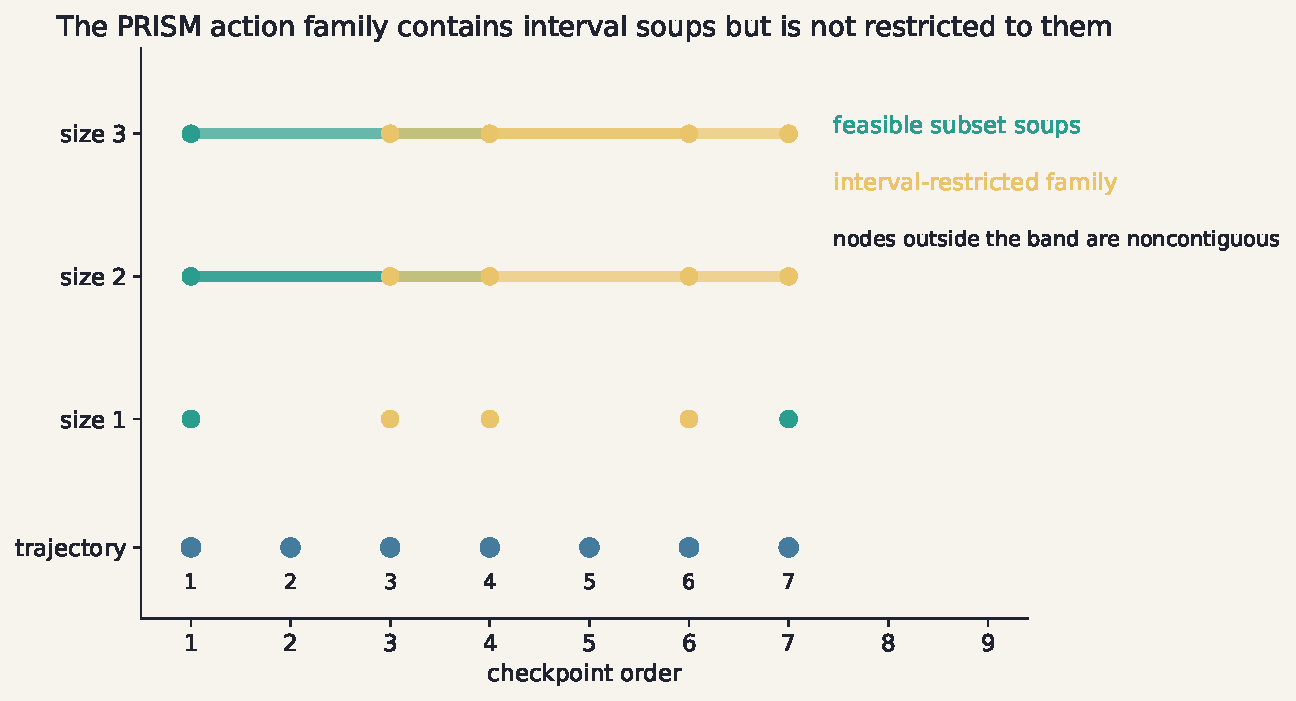
\includegraphics[width=0.86\linewidth]{figures/action_family_vs_interval_band.pdf}
    \caption{\textbf{Action-family view.} Interval-restricted selectors operate on a strict subfamily of the feasible subset soups available to \prism{}. The theory compares these methods at the level of the shared certificate rather than via a claim of universal empirical dominance.}
    \label{fig:action_family}
\end{figure}

\subsection{Consistency over a finite action class}

Conditional on a fixed candidate pool after the validation stage, the post-hoc action family \(\cS_M\) is finite. This makes consistency of the second-stage selector straightforward once the empirical objective is written as a finite max of pairwise empirical-\(\CVaR\) gaps.

\begin{assumption}[Bounded measurable action losses]
\label{ass:bounded_losses}
For every feasible action \(S\in\cS_M\), the loss \(\loss(Z;S)\) is measurable and bounded in \([0,L_{\max}]\).
\end{assumption}

\begin{theorem}[Consistency of the second-stage selector conditional on a fixed candidate family]
\label{thm:consistency}
Suppose Assumption~\ref{ass:bounded_losses} holds and \(\cS_M\) is treated as fixed after the validation-stage candidate construction. Let \(\widehat{\Psi}_\alpha\) be the empirical objective in Eq.~\eqref{eq:empirical_prism} built from an \iid{} support sample \(Z_1,\ldots,Z_n \sim P\), and let \(\Psi_\alpha\) be the population objective in Eq.~\eqref{eq:population_prism}. Then
\begin{equation}
    \sup_{S\in\cS_M}
    \left|
        \widehat{\Psi}_\alpha(S) - \Psi_\alpha(S)
    \right|
    \xrightarrow[]{a.s.} 0
    \qquad \text{as } n\to\infty.
    \label{eq:uniform_consistency}
\end{equation}
\end{theorem}

\begin{corollary}[Eventual identification under a population gap]
\label{cor:identification}
If the population minimizer \(S_\alpha^\star\) is unique and satisfies
\begin{equation}
    \inf_{S\neq S_\alpha^\star}
    \bracks{
        \Psi_\alpha(S) - \Psi_\alpha(S_\alpha^\star)
    }
    > 0,
    \label{eq:population_gap}
\end{equation}
then the empirical minimizer \(\widehat{S}_\alpha\) equals \(S_\alpha^\star\) eventually almost surely.
\end{corollary}

\subsection{Monotonic robustness certificates}

The subpopulation size parameter \(\alpha\) has a direct robustness interpretation. Smaller \(\alpha\) permits sharper reweightings and is therefore harder to protect.

\begin{proposition}[Monotonicity in \(\alpha\)]
\label{prop:alpha_monotone}
For every fixed action \(S\in\cS_M\), the map \(\alpha \mapsto \Psi_\alpha(S)\) is nonincreasing on \((0,1]\). Equivalently, if \(0 < \alpha_1 \le \alpha_2 \le 1\), then
\begin{equation}
    \Psi_{\alpha_1}(S) \ge \Psi_{\alpha_2}(S).
    \label{eq:alpha_monotonicity}
\end{equation}
\end{proposition}

This motivates a certificate of subgroup robustness at a fixed regret tolerance \(\tau_{\mathrm{reg}}>0\):
\begin{equation}
    \alpha_\tau^\star(S)
    \triangleq
    \inf\braces{
        \alpha\in(0,1] :
        \Psi_\alpha(S)\le \tau_{\mathrm{reg}}
    }.
    \label{eq:alpha_star}
\end{equation}
Smaller \(\alpha_\tau^\star(S)\) indicates that \(S\) remains near-optimal even for relatively small hidden subpopulations.

\begin{figure}[t]
    \centering
    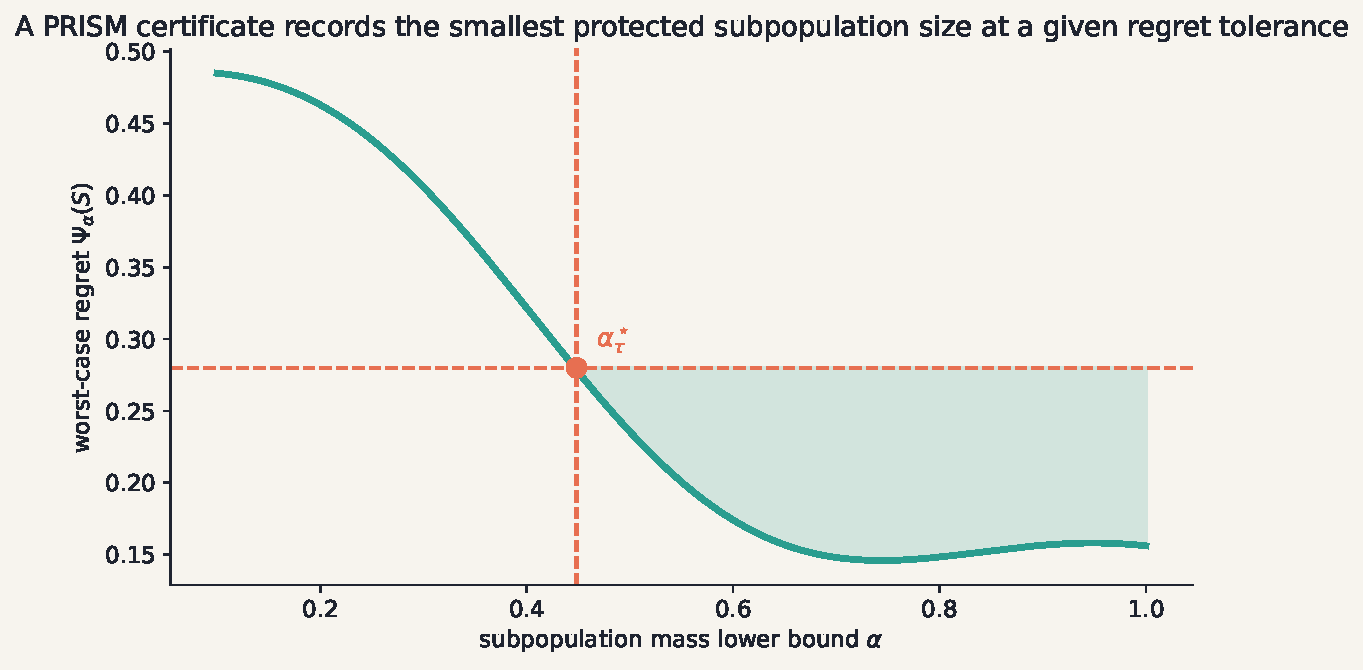
\includegraphics[width=0.78\linewidth]{figures/certificate_curve_alpha_star.pdf}
    \caption{\textbf{Certificate interpretation.} Because \(\Psi_\alpha(S)\) is monotone in \(\alpha\), each soup admits a robustness threshold \(\alpha_\tau^\star\) for any chosen regret tolerance.}
    \label{fig:certificate}
\end{figure}

\subsection{Why complementarity and noncontiguity can be necessary}

The next results formalize two motivations for subset soups: complementarity across latent subpopulations and the need to escape contiguous intervals.

\begin{theorem}[Complementary subgroup-specialized checkpoints]
\label{thm:complementarity}
Assume the support distribution \(P\) is partitioned into \(K\) hidden subpopulations \(G_1,\ldots,G_K\) of equal mass \(1/K\), with \(\alpha \le 1/K\). Suppose there exist \(K\) feasible checkpoints \(t_1,\ldots,t_K\in\cC\) such that for some \(L>0\),
\begin{equation}
    \loss(Z;t_k)
    =
    \begin{cases}
        0, & Z\in G_k,\\
        L, & Z\in G_j,\; j\neq k,
    \end{cases}
    \label{eq:specialized_losses}
\end{equation}
and suppose uniform soups average these losses exactly:
\begin{equation}
    \loss(Z;S)
    =
    \frac{1}{|S|}
    \sum_{t\in S} \loss(Z;t)
    \qquad \forall S\subseteq\braces{t_1,\ldots,t_K}.
    \label{eq:exact_soup_average}
\end{equation}
Then the full complementary soup \(S_{\mathrm{all}}=\braces{t_1,\ldots,t_K}\) satisfies
\begin{equation}
    \Psi_\alpha(S_{\mathrm{all}})
    =
    L\paren{1-\frac{1}{K}},
    \label{eq:full_soup_regret}
\end{equation}
whereas every proper subset \(S\subsetneq S_{\mathrm{all}}\) satisfies
\begin{equation}
    \Psi_\alpha(S)=L.
    \label{eq:incomplete_soup_regret}
\end{equation}
Therefore \prism{} strictly prefers the full complementary soup.
\end{theorem}

Theorem~\ref{thm:complementarity} gives a precise notion of useful complementarity. If different checkpoints specialize to different hidden subpopulations and the soup remains local enough for uniform averaging to make sense, then the regret-optimal soup includes all of them.

\begin{proposition}[Constructive noncontiguous separation]
\label{prop:noncontiguous}
There exists a trajectory order \(1<2<3<4\), a feasible action family with \(M=4\), and hidden subpopulations \(A,B\) of equal mass such that the noncontiguous pair \(S^\dagger = \braces{1,4}\) satisfies
\begin{equation}
    \Psi_{1/2}(S^\dagger)=2,
    \label{eq:noncontig_value}
\end{equation}
while every singleton and every contiguous interval \(I\) satisfies
\begin{equation}
    \Psi_{1/2}(I) > 2.
    \label{eq:interval_worse}
\end{equation}
One explicit construction is given by checkpoint losses
\begin{equation}
    \loss(\cdot;1)=(0,4),\quad
    \loss(\cdot;2)=(4,4),\quad
    \loss(\cdot;3)=(4,4),\quad
    \loss(\cdot;4)=(4,0),
    \label{eq:noncontiguous_example}
\end{equation}
with soup losses defined by uniform averaging.
\end{proposition}

\begin{figure}[t]
    \centering
    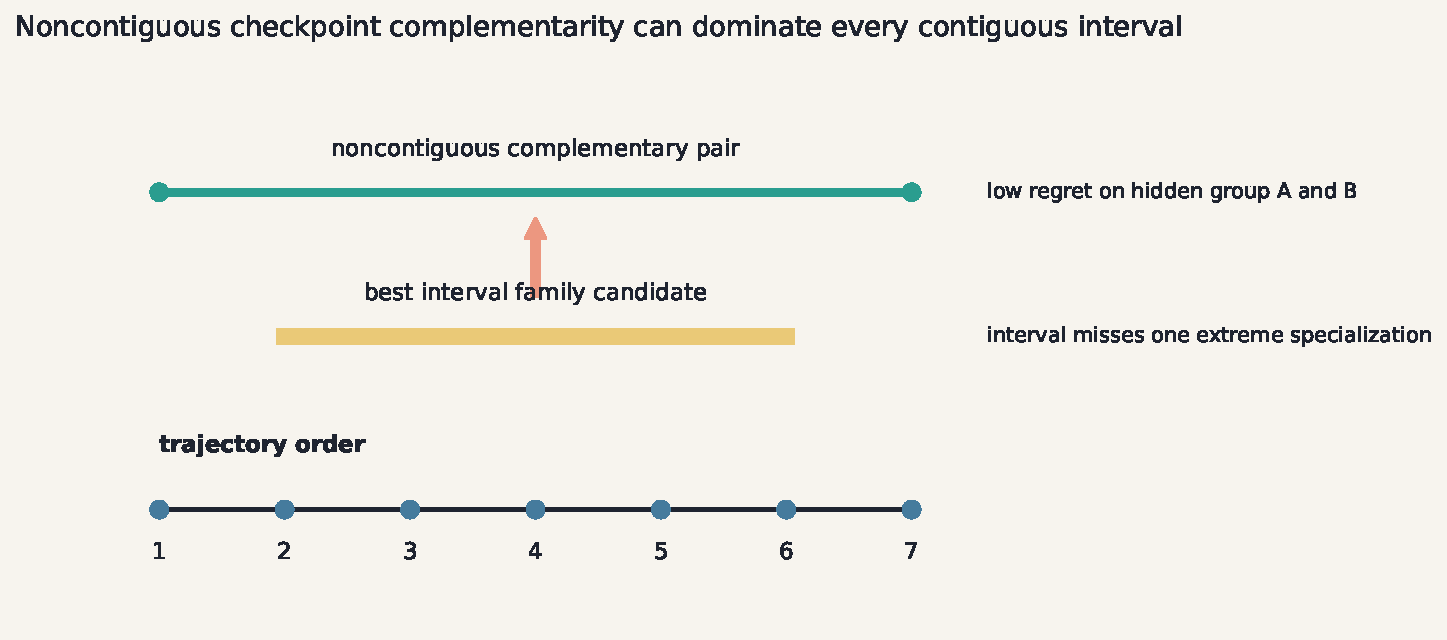
\includegraphics[width=0.87\linewidth]{figures/noncontiguous_complementarity.pdf}
    \caption{\textbf{Noncontiguous separation.} Even when every contiguous interval is feasible, the regret-optimal soup can require checkpoints from distant parts of the trajectory because those checkpoints specialize to different hidden subpopulations.}
    \label{fig:noncontiguous}
\end{figure}

\subsection{Why regret rather than raw risk}

Regret is the right primitive here for the same reason it is attractive in robust learning under heterogeneous shift: raw risk mixes subgroup difficulty with excess loss. If two hidden subpopulations differ in irreducible noise or inherent difficulty, minimizing worst-case raw risk can favor uniformly conservative soups even when another feasible soup is much closer to the subgroup-wise optimum. Regret removes the subgroup-specific floor by comparing each candidate soup only to the best feasible soup for that subpopulation.

\begin{figure}[t]
    \centering
    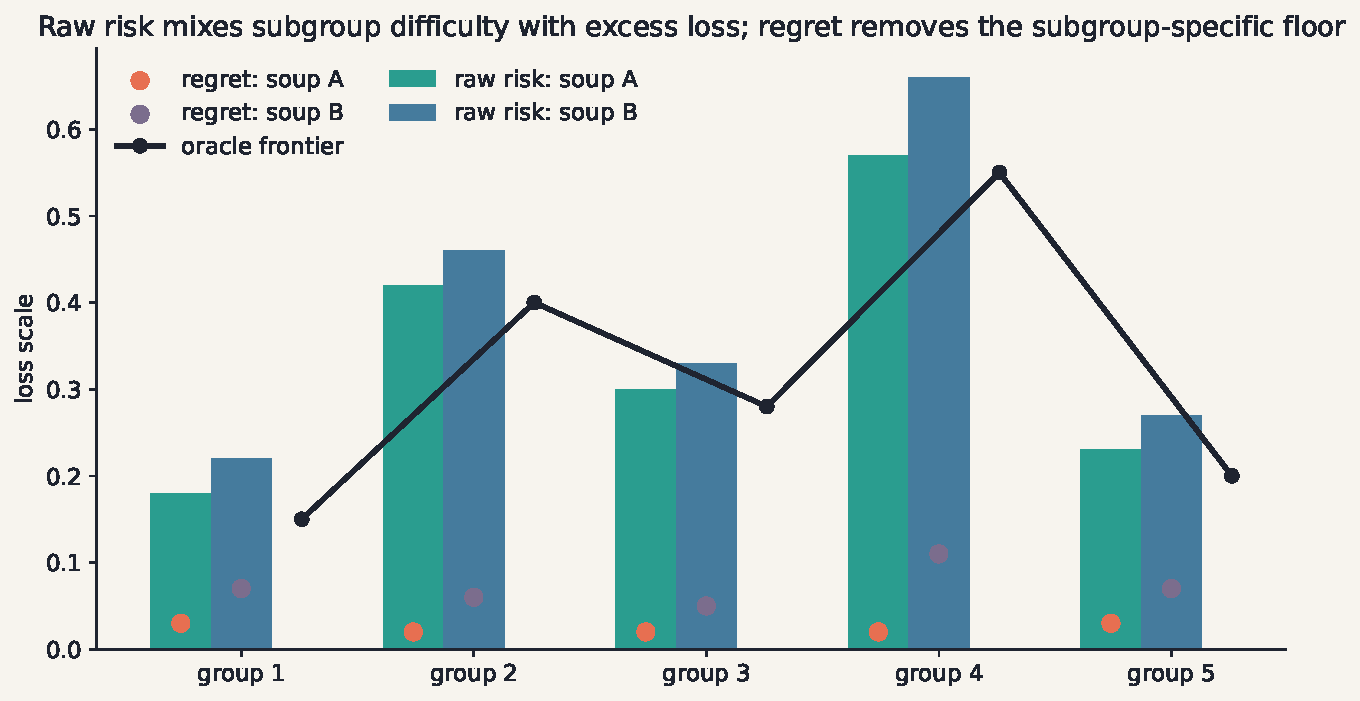
\includegraphics[width=0.86\linewidth]{figures/risk_vs_regret_noise.pdf}
    \caption{\textbf{Raw risk versus regret.} Raw subgroup risk combines irreducible subgroup difficulty with excess loss. Regret isolates the performance gap to the best feasible soup on each subgroup.}
    \label{fig:risk_regret}
\end{figure}

\section{Experimental Protocol and Published Context}
\label{sec:experiments}

This section fixes the experimental protocol and records exact published benchmark numbers from prior work. Tables~\ref{tab:prism_tbd} and \ref{tab:ablation_tbd} reserve the reporting structure for the new empirical measurements.

\subsection{Protocol}

The evaluation protocol follows the standard DomainBed setup \citep{gulrajani2021domainbed} on PACS, VLCS, OfficeHome, TerraIncognita, and DomainNet using the canonical leave-one-domain-out split. The base model is a dense single-run source-pooled learner, and all post-hoc selectors operate on checkpoints from that one run. The held-out pooled source data are split into a validation subset for candidate-pool construction and a support subset for post-hoc selection. The primary metric is mean test-domain accuracy over the standard held-out target domains.

The planned comparisons include:
\begin{itemize}[leftmargin=1.4em]
    \item plain \erm{},
    \item published interval-based post-hoc selectors,
    \item diverse or locality-aware weight-averaging methods,
    \item pretraining-aware DG methods with and without post-hoc selectors,
    \item and ablations of \prism{} over \(\alpha\), \(M\), \(\varepsilon\), \(\tau\), and the candidate-pool construction.
\end{itemize}

\subsection{Published benchmark context}

Table~\ref{tab:published_context} records exact published numbers that define the current post-hoc DG context. These values are copied from the original papers and kept in their original reporting styles.

\begin{table}[t]
    \centering
    \small
    \caption{\textbf{Published DomainBed context from prior work.} The upper block reproduces the single-number reporting style of \citet{cha2021swad}; the lower block reproduces the mean\(\pm\)stderr reporting style of \citet{cha2022miro}.}
    \label{tab:published_context}
    \setlength{\tabcolsep}{5pt}
    \begin{tabular}{lcccccc}
        \toprule
        Method & PACS & VLCS & OfficeHome & TerraInc & DomainNet & Avg. \\
        \midrule
        \erm{} \citep{cha2021swad} & 85.5 & 77.5 & 66.5 & 46.1 & 40.9 & 63.3 \\
        \swad{} \citep{cha2021swad} & 88.1 & 79.1 & 70.6 & 50.0 & 46.5 & 66.9 \\
        CORAL + \swad{} \citep{cha2021swad} & 88.3 & 78.9 & 71.3 & 51.0 & 46.8 & 67.3 \\
        \midrule
        \miro{} \citep{cha2022miro} & \(85.4\pm0.4\) & \(79.0\pm0.0\) & \(70.5\pm0.4\) & \(50.4\pm1.1\) & \(44.3\pm0.2\) & 65.9 \\
        \miro{} + \swad{} \citep{cha2022miro} & \(88.4\pm0.1\) & \(79.6\pm0.2\) & \(72.4\pm0.1\) & \(52.9\pm0.2\) & \(47.0\pm0.0\) & 68.1 \\
        \bottomrule
    \end{tabular}
\end{table}

\subsection{\prism{} reporting tables}

\begin{table}[t]
    \centering
    \small
    \caption{\textbf{Primary \prism{} reporting table.}}
    \label{tab:prism_tbd}
    \setlength{\tabcolsep}{7pt}
    \begin{tabular}{lcccccc}
        \toprule
        Method & PACS & VLCS & OfficeHome & TerraInc & DomainNet & Avg. \\
        \midrule
        \prism{} & \TBD & \TBD & \TBD & \TBD & \TBD & \TBD \\
        \prism{} + stronger backbone & \TBD & \TBD & \TBD & \TBD & \TBD & \TBD \\
        \prism{} + pretrained base & \TBD & \TBD & \TBD & \TBD & \TBD & \TBD \\
        \bottomrule
    \end{tabular}
\end{table}

\begin{table}[t]
    \centering
    \small
    \caption{\textbf{\prism{} ablation table.}}
    \label{tab:ablation_tbd}
    \setlength{\tabcolsep}{8pt}
    \begin{tabular}{lccc}
        \toprule
        Variant & PACS & Avg. & Comment \\
        \midrule
        \prism{} baseline & \TBD & \TBD & exact selector \\
        Smaller \(\alpha\) & \TBD & \TBD & stronger hidden-subpopulation adversary \\
        Larger \(M\) & \TBD & \TBD & broader soup family \\
        No barrier filter & \TBD & \TBD & locality ablation \\
        Interval-only family & \TBD & \TBD & restricted action class \\
        \bottomrule
    \end{tabular}
\end{table}

\section{Discussion}

\prism{} is intentionally narrow. It does not claim to solve DG in full generality. The theoretical statement is conditional on source-supported hidden-subpopulation shift: the target distribution must be representable as a bounded reweighting of the pooled source-support distribution. The barrier screen is likewise an explicit modeling choice; it is an anchor-based locality heuristic rather than a certificate that every subset soup remains in one common basin.

Those restrictions are deliberate. One recurring limitation of heuristic post-hoc selectors is that the motivating theory and the scoring stage need not act on the same object. Here the action family is written directly in terms of scored soups and evaluated through regret to the best feasible soup under hidden source-supported shifts. When the assumptions hold, the resulting certificate speaks directly about the scored selector family.

This viewpoint also suggests several future directions. The exhaustive selector is exact but combinatorial. Larger action families may require column generation or branch-and-bound without changing the objective. The current paper studies uniform soups because they align exactly with the scored averaged-state family and avoid an additional weighting surrogate. Finally, the subgroup-support family can be extended to attribute-aware or semantically clustered hidden subpopulations while remaining domain-label-free.

\section*{Acknowledgments}

This section is intentionally omitted for anonymous review.

\bibliographystyle{plainnat}
\bibliography{references}

\appendix

\section{Proofs}

\subsection{Proof of Proposition~\ref{prop:top_alpha}}

\begin{proof}
Fix \(S\in\cS_M\). Starting from Eq.~\eqref{eq:empirical_prism},
\begin{align}
    \widehat{\Psi}_\alpha(S)
    &=
    \sup_{q\in\cQ_\alpha^n}
    \left[
        \sum_{i=1}^{n} q_i \loss_i(S)
        -
        \min_{S'\in\cS_M}
        \sum_{i=1}^{n} q_i \loss_i(S')
    \right] \nonumber\\
    &=
    \sup_{q\in\cQ_\alpha^n}
    \max_{S'\in\cS_M}
    \sum_{i=1}^{n} q_i\paren{\loss_i(S)-\loss_i(S')} \nonumber\\
    &=
    \max_{S'\in\cS_M}
    \sup_{q\in\cQ_\alpha^n}
    \sum_{i=1}^{n} q_i\paren{\loss_i(S)-\loss_i(S')},
    \label{eq:proof_topalpha_swap}
\end{align}
because the outer maximization is over a finite action family and the inner expression is linear in \(q\). This proves Eq.~\eqref{eq:prism_top_alpha}.

Now fix any \(v\in\RR^n\) and consider \(\Top_\alpha(v)\). The feasible set \(\cQ_\alpha^n\) is a compact polytope, and the objective \(q\mapsto q^\top v\) is linear. Hence the supremum is attained at an extreme point of \(\cQ_\alpha^n\). Let \(m=\alpha n\), \(k=\lfloor m\rfloor\), and \(\rho=m-k\).

If \(m\le 1\), the cap \(q_i\le 1/m\) is at least \(1\), so the simplex constraint alone forces the optimizer to place all mass on one coordinate with largest value. Thus \(\Top_\alpha(v)=v_{(1)}\).

If \(m\ge n\), then \(\alpha \ge 1\), so \(q_i \le 1/n\) for every \(i\). Combined with \(\sum_i q_i=1\), this forces \(q_i=1/n\) for all \(i\), giving \(\Top_\alpha(v)=n^{-1}\sum_i v_i\).

Now consider \(1<m<n\). Since each coordinate is capped by \(1/m\), the optimizer saturates the largest entries first. Precisely, there is an optimal \(q^\star\) such that
\[
    q^\star_{(1)}=\cdots=q^\star_{(k)}=\frac{1}{m},\qquad
    q^\star_{(k+1)}=\frac{\rho}{m},\qquad
    q^\star_{(j)}=0 \;\; \text{for } j\ge k+2.
\]
The mass constraint is satisfied because \(k/m+\rho/m = 1\). Substituting this optimizer yields Eq.~\eqref{eq:top_alpha_closed}.

For Eq.~\eqref{eq:top_alpha_cvar}, write the Lagrangian for the constrained optimization
\[
    \sup_{q\ge 0,\;\sum q_i=1,\; q_i\le \frac{1}{\alpha n}} q^\top v.
\]
Introducing a multiplier \(\eta\) for the equality constraint and slack multipliers for the upper bounds, standard linear-program duality yields
\[
    \Top_\alpha(v)
    =
    \inf_{\eta\in\RR}
    \left[
        \eta + \frac{1}{\alpha n}\sum_{i=1}^{n}(v_i-\eta)_+
    \right].
\]
This is exactly the empirical-\(\CVaR\) representation.
\end{proof}

\subsection{Proof of Proposition~\ref{prop:global_optimality}}

\begin{proof}
Algorithm~\ref{alg:prism} explicitly enumerates every feasible action \(S\in\cS_M\), computes its exact empirical objective \(\widehat{\Psi}_\alpha(S)\), and returns an action with smallest value. Therefore it returns a global minimizer of Eq.~\eqref{eq:empirical_prism}.

The action count in Eq.~\eqref{eq:action_count} is immediate from the definition of \(\cS_M\): for each \(m\in\{1,\ldots,M\}\), there are \(\binom{|\cC|}{m}\) feasible actions of size \(m\).

After the candidate pool is fixed, each ordered action pair \((S,S')\) requires computing a top-\(\alpha\) mean over \(n\) support examples. If one treats each top-\(\alpha\) computation as \(O(n)\), then evaluating all ordered pairs requires \(O(n|\cS_M|^2)\) time. This dominates the action-pair regret stage.
\end{proof}

\subsection{Proof of Theorem~\ref{thm:certificate}}

\begin{proof}
Fix \(S\in\cS_M\) and \(r\in\cR_\alpha\). By definition,
\[
    \operatorname{Reg}_r(S)
    =
    \EE_{P_r}[\loss(Z;S)]
    -
    \min_{S'\in\cS_M} \EE_{P_r}[\loss(Z;S')].
\]
But \(\Psi_\alpha(S)\) is the supremum of the same quantity over all \(r'\in\cR_\alpha\). Therefore
\[
    \operatorname{Reg}_r(S) \le \sup_{r'\in\cR_\alpha} \operatorname{Reg}_{r'}(S) = \Psi_\alpha(S),
\]
which proves Eq.~\eqref{eq:certificate_basic}.

If \(S_\alpha^\star\) minimizes \(\Psi_\alpha\) over \(\cS_M\), then for any \(r\in\cR_\alpha\),
\[
    \operatorname{Reg}_r(S_\alpha^\star)
    \le
    \Psi_\alpha(S_\alpha^\star)
    =
    \inf_{S\in\cS_M}\Psi_\alpha(S),
\]
which proves Eq.~\eqref{eq:certificate_minimized}.
\end{proof}

\subsection{Proof of Corollary~\ref{cor:interval_domination}}

\begin{proof}
Because \(\cI_M\subseteq\cS_M\),
\[
    \inf_{S\in\cS_M}\Psi_\alpha(S)
    \le
    \inf_{S\in\cI_M}\Psi_\alpha(S).
\]
Since \(S_\alpha^\star\) minimizes \(\Psi_\alpha\) over \(\cS_M\), the left-hand side equals \(\Psi_\alpha(S_\alpha^\star)\), proving Eq.~\eqref{eq:interval_domination}. Equation~\eqref{eq:interval_domination_target} then follows by combining Theorem~\ref{thm:certificate} with Eq.~\eqref{eq:interval_domination}.
\end{proof}

\subsection{Proof of Theorem~\ref{thm:consistency}}

\begin{proof}
For each ordered pair \((S,S')\in\cS_M\times\cS_M\), define the bounded random variable
\[
    \Delta_{S,S'}(Z) \triangleq \loss(Z;S)-\loss(Z;S') \in [-L_{\max},L_{\max}].
\]
By Proposition~\ref{prop:top_alpha},
\begin{align}
    \Psi_\alpha(S)
    &=
    \max_{S'\in\cS_M}
    \inf_{\eta\in\RR}
    \left[
        \eta + \frac{1}{\alpha}\EE\paren{\Delta_{S,S'}(Z)-\eta}_+
    \right],
    \label{eq:population_cvar_pair}
    \\
    \widehat{\Psi}_\alpha(S)
    &=
    \max_{S'\in\cS_M}
    \inf_{\eta\in\RR}
    \left[
        \eta + \frac{1}{\alpha n}\sum_{i=1}^{n}\paren{\Delta_{S,S'}(Z_i)-\eta}_+
    \right].
    \label{eq:empirical_cvar_pair}
\end{align}
Because \(\Delta_{S,S'}\in[-L_{\max},L_{\max}]\), the infimum over \(\eta\) may be restricted to \([-L_{\max},L_{\max}]\): outside this interval, the objective is strictly larger than its value at the closest endpoint.

Now fix one ordered pair \((S,S')\). The class of functions
\[
    \mathcal{G}_{S,S'}
    \triangleq
    \braces{
        z \mapsto \paren{\Delta_{S,S'}(z)-\eta}_+ :
        \eta\in[-L_{\max},L_{\max}]
    }
\]
is parameterized by a compact interval. For any \(\varepsilon>0\), choose a finite grid
\[
    \Gamma_\varepsilon \subset [-L_{\max},L_{\max}]
\]
with mesh at most \(\varepsilon\). For every fixed \(\eta_0\in\Gamma_\varepsilon\), the strong law of large numbers gives
\[
    \frac{1}{n}\sum_{i=1}^{n}\paren{\Delta_{S,S'}(Z_i)-\eta_0}_+
    -
    \EE\paren{\Delta_{S,S'}(Z)-\eta_0}_+
    \xrightarrow[]{a.s.} 0.
\]
Because \(\Gamma_\varepsilon\) is finite, taking the maximum over grid points preserves almost-sure convergence:
\[
    \max_{\eta_0\in\Gamma_\varepsilon}
    \left|
        \frac{1}{n}\sum_{i=1}^{n}\paren{\Delta_{S,S'}(Z_i)-\eta_0}_+
        -
        \EE\paren{\Delta_{S,S'}(Z)-\eta_0}_+
    \right|
    \xrightarrow[]{a.s.} 0.
\]
Now let \(\eta\in[-L_{\max},L_{\max}]\) and choose \(\eta_0\in\Gamma_\varepsilon\) with \(|\eta-\eta_0|\le \varepsilon\). Since \(u\mapsto(u-\eta)_+\) is 1-Lipschitz in \(\eta\),
\[
    \left|
        (\Delta-\eta)_+ - (\Delta-\eta_0)_+
    \right|
    \le
    |\eta-\eta_0|
    \le
    \varepsilon
\]
pointwise. Therefore
\begin{align*}
    &\sup_{\eta\in[-L_{\max},L_{\max}]}
    \left|
        \frac{1}{n}\sum_{i=1}^{n}\paren{\Delta_{S,S'}(Z_i)-\eta}_+
        -
        \EE\paren{\Delta_{S,S'}(Z)-\eta}_+
    \right| \\
    &\qquad\le
    \max_{\eta_0\in\Gamma_\varepsilon}
    \left|
        \frac{1}{n}\sum_{i=1}^{n}\paren{\Delta_{S,S'}(Z_i)-\eta_0}_+
        -
        \EE\paren{\Delta_{S,S'}(Z)-\eta_0}_+
    \right|
    + 2\varepsilon.
\end{align*}
Taking \(n\to\infty\) and then \(\varepsilon\downarrow 0\) shows that the left-hand side converges to \(0\) almost surely. Therefore, for each fixed pair \((S,S')\),
\[
    \left|
        \inf_{\eta}
        \bracks{
            \eta + \frac{1}{\alpha n}\sum_{i=1}^{n}\paren{\Delta_{S,S'}(Z_i)-\eta}_+
        }
        -
        \inf_{\eta}
        \bracks{
            \eta + \frac{1}{\alpha}\EE\paren{\Delta_{S,S'}(Z)-\eta}_+
        }
    \right|
    \xrightarrow[]{a.s.} 0.
\]
The action family \(\cS_M\) is finite, so the convergence is uniform over all ordered pairs:
\[
    \sup_{S,S'\in\cS_M}
    \left|
        \widehat{R}_\alpha(S,S')
        -
        R_\alpha(S,S')
    \right|
    \xrightarrow[]{a.s.} 0,
\]
where \(\widehat{R}_\alpha(S,S')\) and \(R_\alpha(S,S')\) denote the empirical and population pairwise top-\(\alpha\) regret terms.

Finally, \(\widehat{\Psi}_\alpha(S)=\max_{S'}\widehat{R}_\alpha(S,S')\) and \(\Psi_\alpha(S)=\max_{S'}R_\alpha(S,S')\). A maximum over finitely many uniformly convergent sequences is uniformly convergent, so
\[
    \sup_{S\in\cS_M}
    \left|
        \widehat{\Psi}_\alpha(S)-\Psi_\alpha(S)
    \right|
    \xrightarrow[]{a.s.} 0.
\]
\end{proof}

\subsection{Proof of Corollary~\ref{cor:identification}}

\begin{proof}
Let
\[
    \gamma
    \triangleq
    \inf_{S\neq S_\alpha^\star}
    \bracks{
        \Psi_\alpha(S)-\Psi_\alpha(S_\alpha^\star)
    }
    > 0.
\]
By Theorem~\ref{thm:consistency}, almost surely there exists \(N\) such that for all \(n\ge N\),
\[
    \sup_{S\in\cS_M}
    \left|
        \widehat{\Psi}_\alpha(S)-\Psi_\alpha(S)
    \right|
    < \frac{\gamma}{3}.
\]
For any \(S\neq S_\alpha^\star\) and \(n\ge N\),
\begin{align*}
    \widehat{\Psi}_\alpha(S)
    &\ge
    \Psi_\alpha(S) - \frac{\gamma}{3}
    \\
    &\ge
    \Psi_\alpha(S_\alpha^\star) + \gamma - \frac{\gamma}{3}
    \\
    &>
    \Psi_\alpha(S_\alpha^\star) + \frac{\gamma}{3}
    \\
    &\ge
    \widehat{\Psi}_\alpha(S_\alpha^\star).
\end{align*}
Thus \(S_\alpha^\star\) is the unique empirical minimizer for all \(n\ge N\), almost surely.
\end{proof}

\subsection{Proof of Proposition~\ref{prop:alpha_monotone}}

\begin{proof}
If \(0 < \alpha_1 \le \alpha_2 \le 1\), then
\[
    \cR_{\alpha_2} \subseteq \cR_{\alpha_1},
\]
because the pointwise cap \(r\le \alpha_2^{-1}\) is stricter than \(r\le \alpha_1^{-1}\). Therefore, for any fixed action \(S\),
\[
    \Psi_{\alpha_2}(S)
    =
    \sup_{r\in\cR_{\alpha_2}} \operatorname{Reg}_r(S)
    \le
    \sup_{r\in\cR_{\alpha_1}} \operatorname{Reg}_r(S)
    =
    \Psi_{\alpha_1}(S).
\]
\end{proof}

\subsection{Proof of Theorem~\ref{thm:complementarity}}

\begin{proof}
Fix the full set \(S_{\mathrm{all}}=\braces{t_1,\ldots,t_K}\). By Eq.~\eqref{eq:exact_soup_average}, for any \(Z\in G_j\),
\[
    \loss(Z;S_{\mathrm{all}})
    =
    \frac{1}{K}
    \left[
        0 + \sum_{k\neq j} L
    \right]
    =
    L\paren{1-\frac{1}{K}}.
\]
The witness action \(t_j\) attains zero loss on \(G_j\), so on subpopulation \(G_j\) the regret of \(S_{\mathrm{all}}\) is \(L(1-1/K)\). Because each \(G_j\) has mass \(1/K\ge \alpha\), the adversary may focus on any one such subgroup, yielding
\[
    \Psi_\alpha(S_{\mathrm{all}})
    =
    L\paren{1-\frac{1}{K}}.
\]

Now take any proper subset \(S\subsetneq S_{\mathrm{all}}\). Then there exists some \(j\) with \(t_j\notin S\). For every \(Z\in G_j\), each checkpoint in \(S\) incurs loss \(L\), so the uniform soup also incurs loss \(L\). Again \(t_j\) is a feasible witness action with zero loss on \(G_j\), hence the regret of \(S\) on \(G_j\) is \(L\). Since the adversary may choose \(G_j\), we have \(\Psi_\alpha(S)\ge L\). The regret can never exceed \(L\) because all action losses lie in \([0,L]\), so \(\Psi_\alpha(S)=L\).

Finally, \(L(1-1/K)<L\), proving that the full complementary soup is strictly preferred.
\end{proof}

\subsection{Proof of Proposition~\ref{prop:noncontiguous}}

\begin{proof}
Assume two hidden subpopulations \(A\) and \(B\), each with mass \(1/2\). Let the four checkpoints have loss vectors
\[
    \loss(\cdot;1)=(0,4),\quad
    \loss(\cdot;2)=(4,4),\quad
    \loss(\cdot;3)=(4,4),\quad
    \loss(\cdot;4)=(4,0),
\]
and let every soup be the uniform average of its member checkpoints.

For the noncontiguous pair \(S^\dagger=\braces{1,4}\), the soup loss is \((2,2)\). On subgroup \(A\), witness action \(1\) attains loss \(0\), so the regret is \(2\). On subgroup \(B\), witness action \(4\) attains loss \(0\), so the regret is also \(2\). Therefore \(\Psi_{1/2}(S^\dagger)=2\).

Now consider contiguous intervals. Every singleton has objective at least \(4\), since checkpoint \(1\) has regret \(4\) on subgroup \(B\), checkpoint \(4\) has regret \(4\) on subgroup \(A\), and checkpoints \(2,3\) have regret \(4\) on both. For the size-two contiguous intervals:
\[
    \braces{1,2}\mapsto (2,4),\qquad
    \braces{2,3}\mapsto (4,4),\qquad
    \braces{3,4}\mapsto (4,2),
\]
whose worst-case regrets are \(4\), \(4\), and \(4\), respectively.

For the size-three contiguous intervals:
\[
    \braces{1,2,3}\mapsto \left(\frac{8}{3},4\right),\qquad
    \braces{2,3,4}\mapsto \left(4,\frac{8}{3}\right),
\]
so their objectives are \(4\). For the full interval \(\braces{1,2,3,4}\), the soup loss is \((3,3)\), so the regret is \(3\) on both subgroups. Hence every contiguous interval has objective strictly larger than \(2\), while the noncontiguous pair \(\braces{1,4}\) has objective \(2\).
\end{proof}

\section{Additional Background from Prior Literature}

For completeness, we record two prior theoretical viewpoints that motivate the present formulation.

\paragraph{Flat minima and DG.}
The flat-minima perspective in DG uses a robust empirical risk over parameter perturbations. In the notation of \citet{cha2021swad}, Theorem 1 bounds the target-domain loss by a robust empirical loss, a source-target divergence term, and a confidence term. Theorem 2 then upper-bounds the DG gap of the robust-risk minimizer by the gap between robust risk minimization and empirical risk minimization, again plus divergence and confidence terms.

\paragraph{Diversity and locality in weight averaging.}
\diwa{} decomposes the expected \ood{} error of weight averaging into bias, variance, covariance, and locality \citep{rame2022diwa}. In their Proposition 1,
\begin{equation}
    \EE\mathcal{E}_T(\theta_{\mathrm{WA}})
    =
    \EE\bracks{
        \operatorname{bias}^2
        + \frac{1}{M}\operatorname{var}
        + \frac{M-1}{M}\operatorname{cov}
    }
    + O(\Delta^2).
    \label{eq:diwa_appendix}
\end{equation}
This viewpoint is complementary to the present paper: locality is encoded in the feasible action family, while complementarity emerges through worst-case regret across hidden subpopulations.

\section{Implementation Details}

The candidate pool is built from dense checkpoints using pooled validation loss and an anchor-based interpolation screen to the best pooled-validation checkpoint. The action family consists of all subsets of size at most \(M\), subject to an explicit action-count guard. The second-stage selector computes support losses for the scored uniform soups, evaluates Eq.~\eqref{eq:prism_top_alpha}, and returns the empirical minimizer when the scored family is fully enumerated. In implementations with batch-normalization layers, the winning soup may then undergo a single post-selection BN refresh before final evaluation.

\end{document}
